\documentclass{article}
\usepackage{graphicx}
\begin{document}


Jorge Torres\\
Universidad de Los Andes\\
Metodos Computacionales Taller 5\\
\vspace{1cm}

\begin{figure}[h!]
  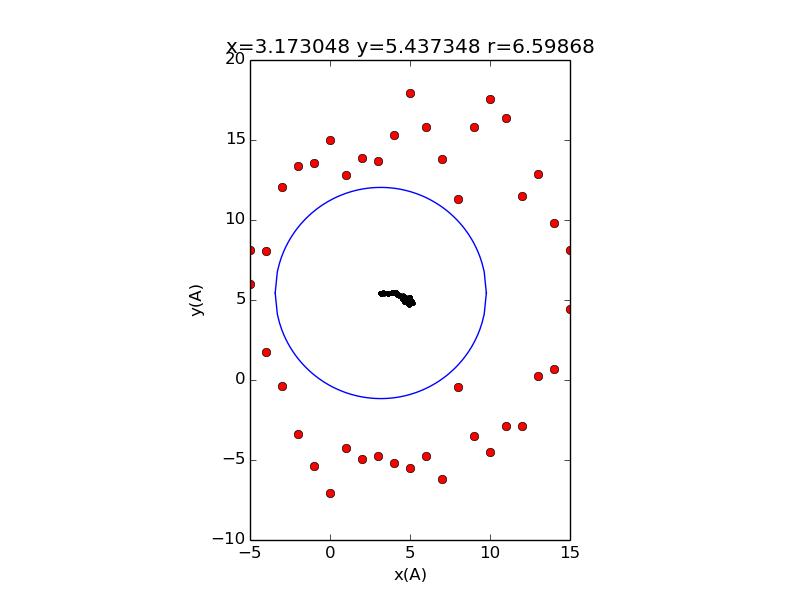
\includegraphics[scale=0.7]{radio_de_poro.png}
  \caption{Caso 1 Radio de poro }
\end{figure}
Podemos observar que el radio del poro es 6.6(A) y es el adecuado para el diametro del poro y la distribucion de los datos. En el centro del circulo se observan vairos puntos negros que representan el centro del ciruclo que se desplaza a la izquierda mientras que encunetra el centro del circulo que mejor se ajusta al metodo de monte carlo\\

\newpage
\begin{figure}[h!]
  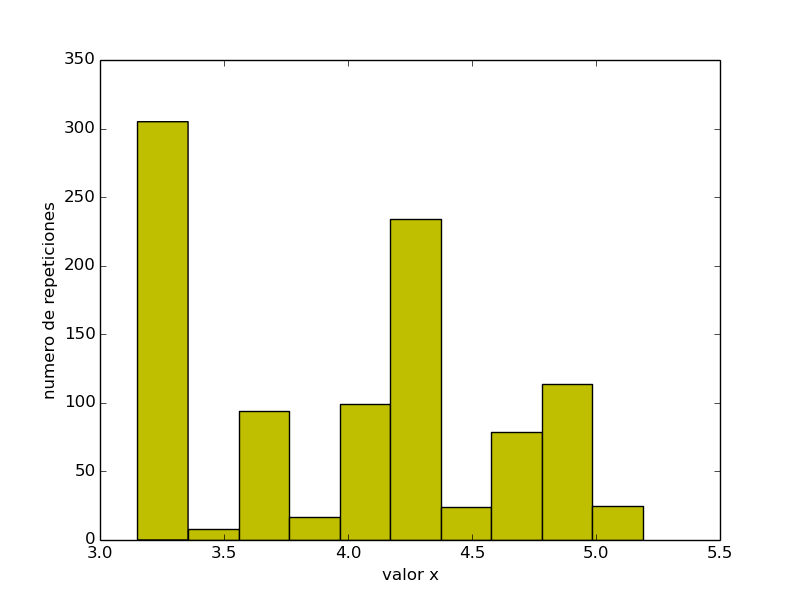
\includegraphics[scale=0.5]{histrogramax.png}
  \caption{Caso 1 Histograma para la distancia x  }
\end{figure}
Vemos que la mejor distancia tiene una mayor cantidad de repeticiones entre 3.1-3.5. Las repeticiones se presentan en un rango de 3-5.4, donde el metodo debe pasar por varios tentativas soluciones al problema, hasta encontrar la mejor de x= 3.173048.\\

\newpage
\begin{figure}[h!]
  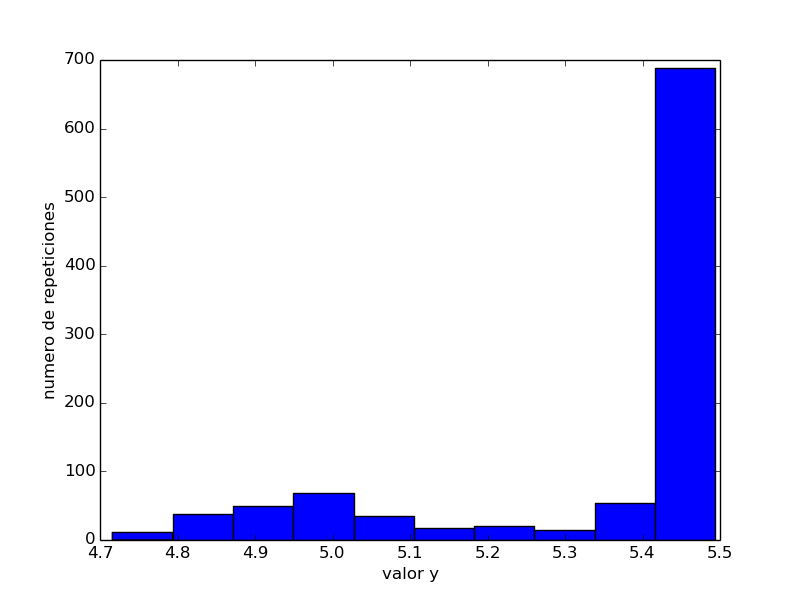
\includegraphics[scale=0.5]{histrogramay.png}
  \caption{Caso 1 Histograma para la distancia y  }
\end{figure}
Vemos que la mejor distancia tiene una mayor cantidad de repeticiones entre 5.4-5.6, y no tiene un rango de aleatoriedad mayor que el de la distancia x, de acuerdo al modelo tentativo, los valores inciales son muy cercanos a los que enconrtramos usando el metodo. La distancia ideal en las coordenadas y es de 5.437348.  \\

\newpage
\begin{figure}[h!]
  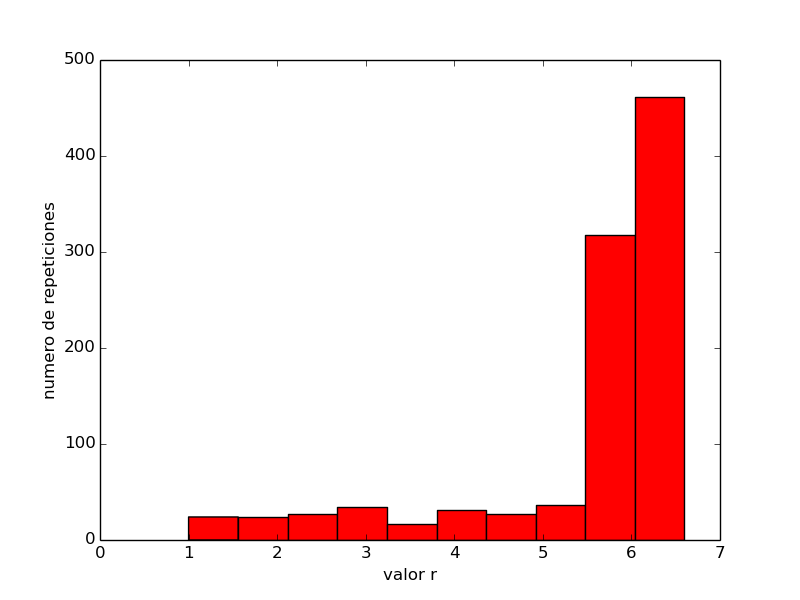
\includegraphics[scale=0.5]{histrogramar.png}
  \caption{Caso 1 Histograma para la distancia r  }
\end{figure}
Vemos que la mejor distancia tiene una mayor cantidad de repeticiones entre 6-7, alrededor de 600 repeticiones, el radio del poro no varia mucho a la hora de encontrar el ideal para la distribucion de datos, en este caso siempre se fue acercando al radio ideal y despues de 5.5 se encuentra facilemente el radio "ideal" de 6.59868, que segun la figura 1 se puede mejor el radio en cantidades muy minusculas.   \\

\newpage
\begin{figure}[h!]
  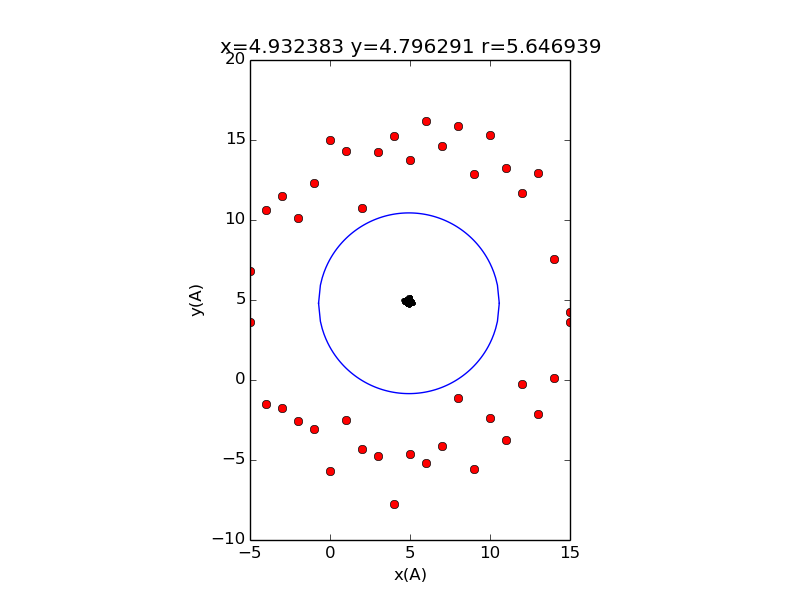
\includegraphics[scale=0.5]{radio_de_poro1.png}
  \caption{Caso 2 Radio de poro 2  }
\end{figure}
A diferencia del primero caso, el centro del radio del poro no cambia tanto ya que segun el punto negro del centro vemos que se mantiene casi constante, lo que cambia es  el radio del poro. \\

\newpage
\begin{figure}[h!]
  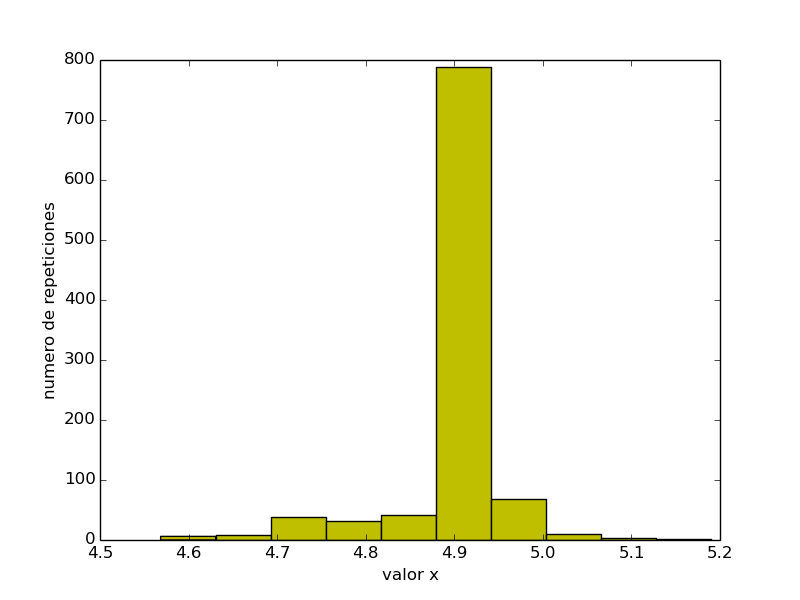
\includegraphics[scale=0.5]{histrogramax1.png}
  \caption{Caso 2 Histograma para la distancia x  }
\end{figure}
Bastante diferente con respecto al histograma en x del caso 1, donde las repeticiones fueron casi constantes en un punto, donde la mejor distancia en la coordenada x es 4.932383 .\\


\newpage
\begin{figure}[h!]
  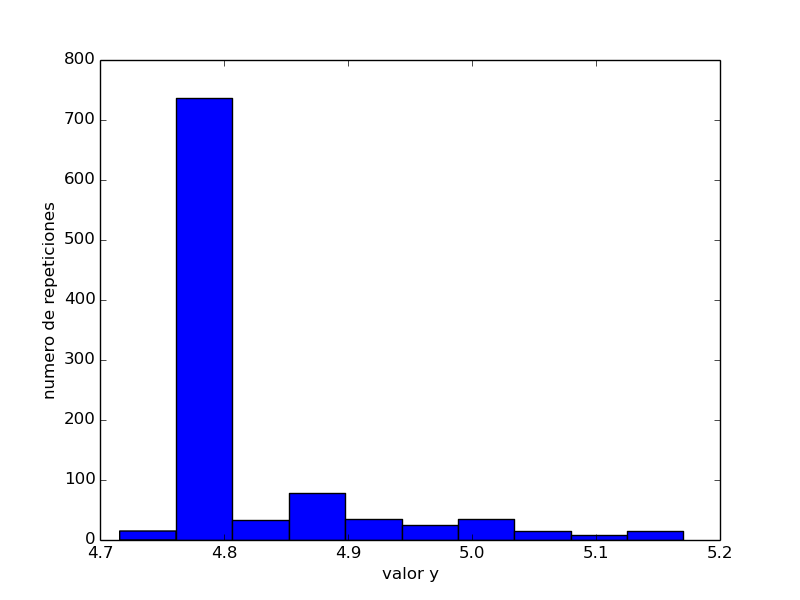
\includegraphics[scale=0.5]{histrogramay1.png}
  \caption{Caso 2 Histograma para la distancia y  }
\end{figure}
Al igual que en las coordenadas del eje x, en el eje y vemos un mismo comportamiento de distribucion en la repeticion de los datos, sin embargo, estos tiene un valor de 4.796291, en el caso 2 se presentan mas numero de repeticiones que en el caso 1. \\


\newpage
\begin{figure}[h!]
  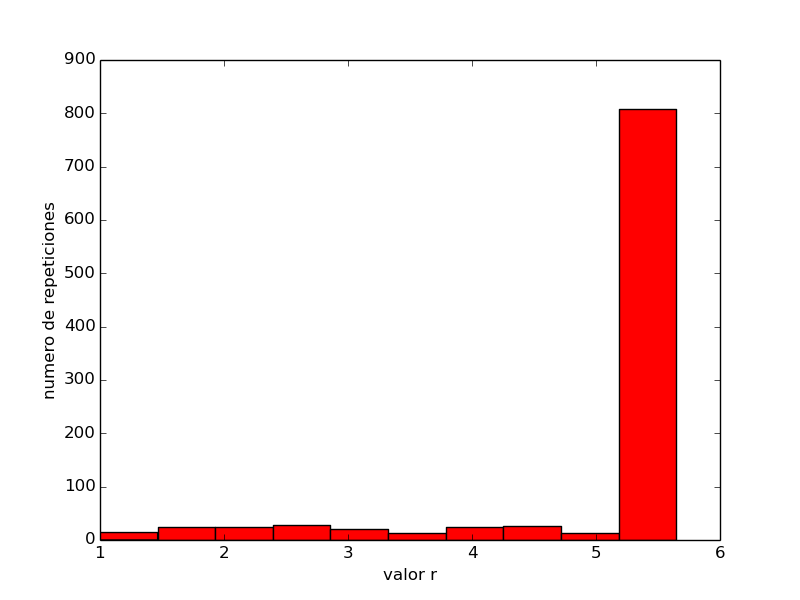
\includegraphics[scale=0.5]{histrogramar1.png}
  \caption{Caso 2 Histograma para la distancia r  }
\end{figure}
Para el caso 2 el radio del poro es de 5.646939 siendo menor que que el caso 1, lo que indica que la distribucion de los puntos en el caso 2 estaban mas cerca y dificultaba el crecimiento del radio del poro.  \\

\newpage
Parte 2 - Carga de un circuito RC\\
\\
\\
\\
\begin{figure}[h!]
  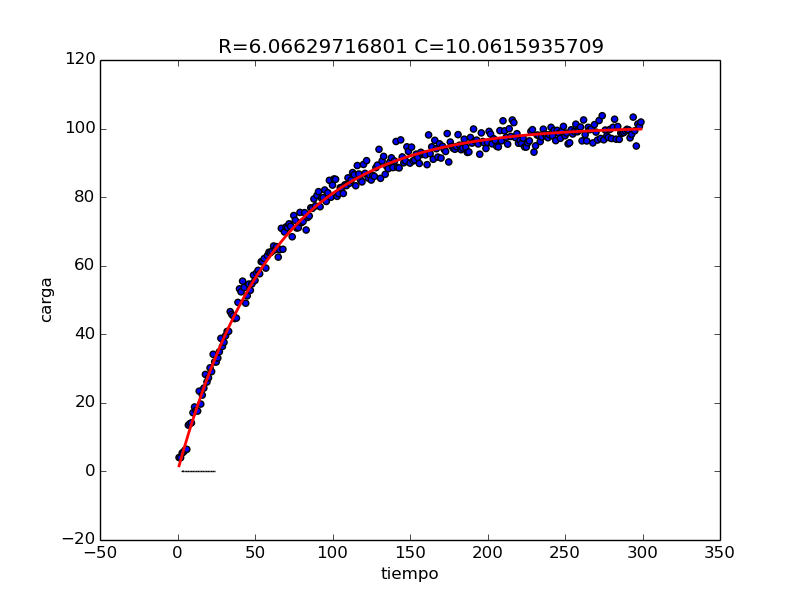
\includegraphics[scale=0.5]{modelo_Vs_datos.png}
  \caption{Caso 1 Modelo Vs Datos   }
\end{figure}
   El modelo obtenido por el metodo de monte carlo se ajusta perfectamente a los datos de observacion, como lo ejemplifica la figura 9. La mejor C es de 10.057 y R de 5.910 que son valores muy cercanos a los valores inciales antes de inciar el recorrido con monte carlo. \\

\newpage
\begin{figure}[h!]
  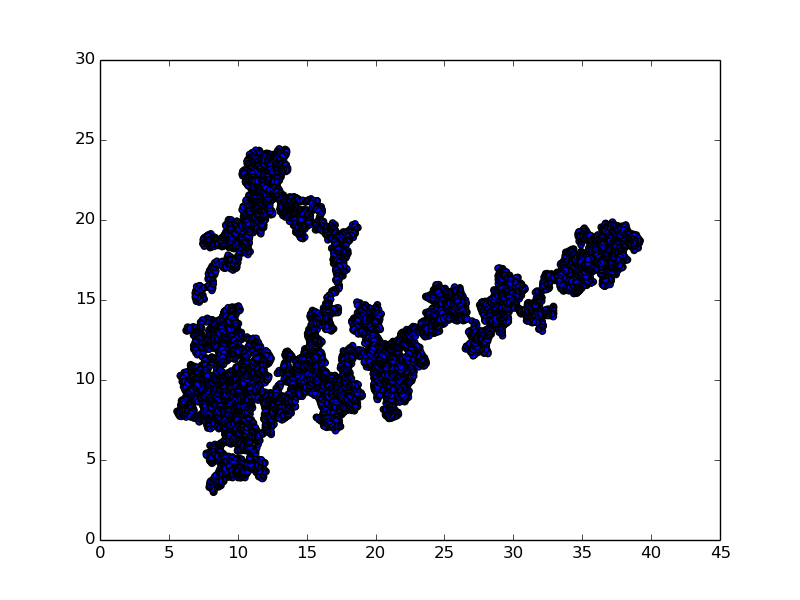
\includegraphics[scale=0.5]{distribucion.png}
  \caption{Caso 1 Distribucion de R y C  }
\end{figure}
se muestra la relacion entre los puntos obtenidos por el metodo de monte carlo y como se agrupan los valors tanto para R y C. \\

\newpage
\begin{figure}[h!]
  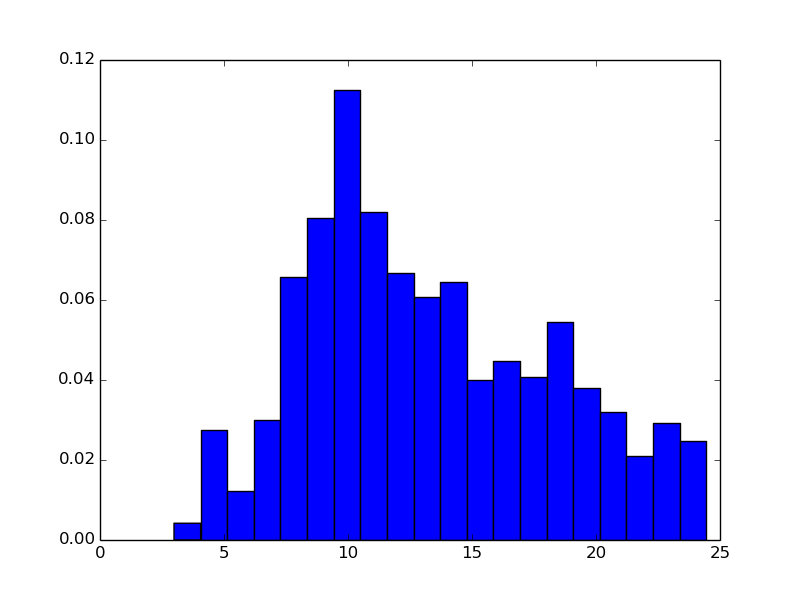
\includegraphics[scale=0.5]{histogramaC.png}
  \caption{Caso 1 Histograma de C }
\end{figure}
El histograma de C nos muestra que la mayor distribucion de puntos esta dado alrededor 15 y se comporta como una campana de Gauss. \\

\newpage
\begin{figure}[h!]
  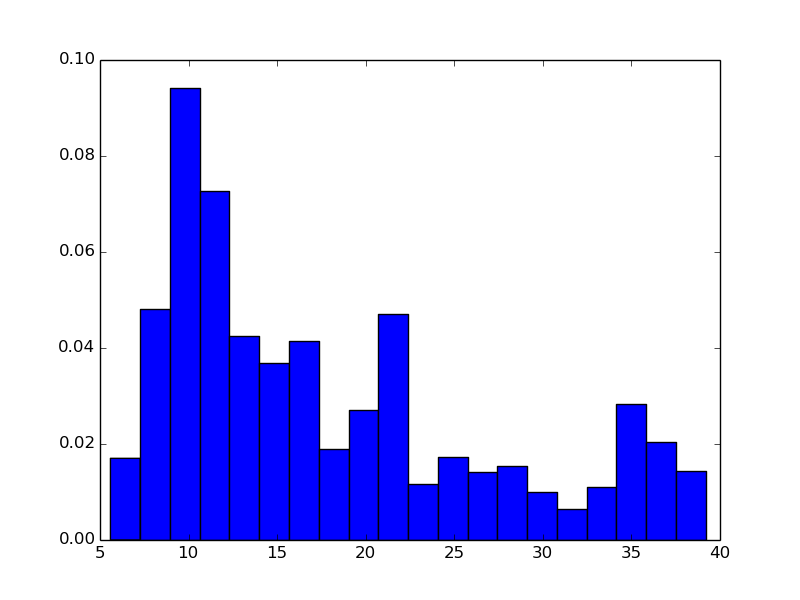
\includegraphics[scale=0.5]{histogramaR.png}
  \caption{Caso 1 Histograma de R }
\end{figure}
El histograma de R nos muestra que la mayor distribucion de puntos que en el caso de C y observamos un comportamiento difernte que para C . \\





% git add --all
% git commit -m 'final'
% gir push 

\end{document}